\section{Prognostics}
\label{sec:prognostics}

A general definition of prognostics is that of a process predicting the time of occurrence of an event $E$ \cite{Daigle2015}. Using notation from Section \ref{sec:systems}, if $\phi_E: S \rightarrow \mathbb{B}$ (where $\mathbb{B} \triangleq \{0,1\}$) is an event threshold function, then $t_E \triangleq \text{inf}\{t \in [t_p,t_p+H]: \phi_E(s_t) = 1\}$ is the nearest predicted time of $E$ ($s_t$ is the state at time $t$). If the state evolution trajectory is non-deterministic, then $p(t_E|s_{0:t_p})$ is computed instead. If states cannot be directly observed, $p(t_E|o_{0:t_p})$ is computed. As defined, prognostics is only meaningful in a specific set of circumstances and next we use two examples to illustrate why.

\subsection{Uncontrolled systems}

There are two main desirable, interrelated attributes for a prognostic system: (1) low uncertainty in EOL estimation, so that a decision about mitigation or recovery actions can be made with confidence, and (2) the ability to make a prediction far enough in advance for the actions to be successfully executed. For uncontrolled systems, this means that prognostics is primarily useful for systems with long lifetimes, low process uncertainty, or both. To illustrate why this is the case, we start with a simple uncontrolled system example:

\begin{figure}[h]
	\centering
		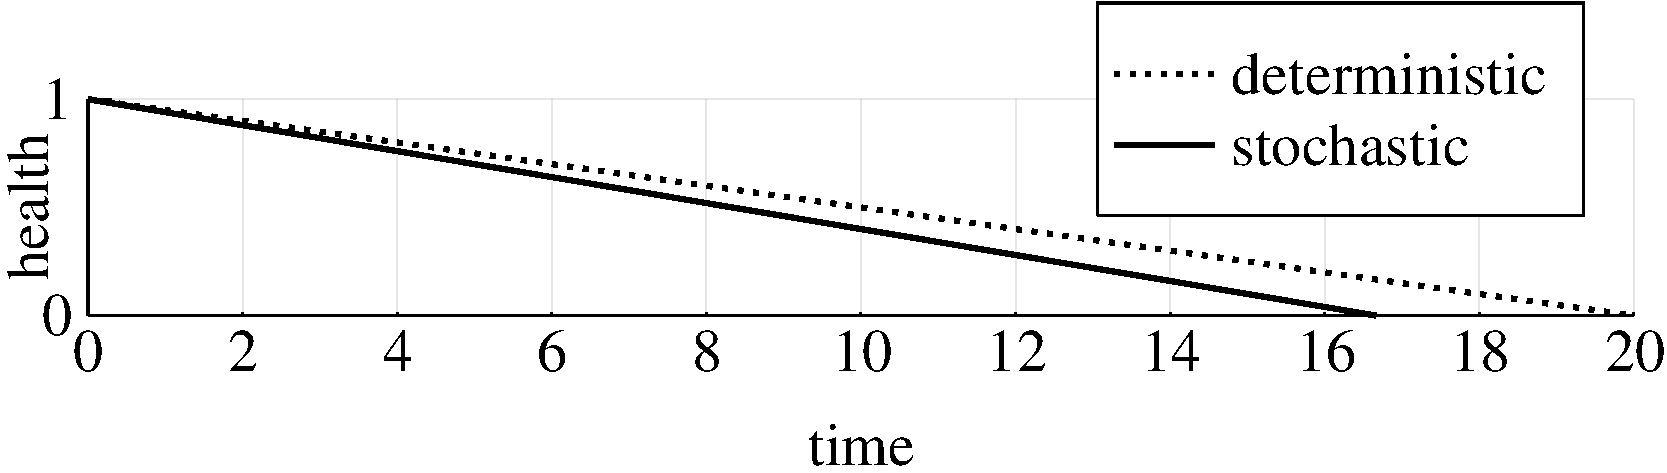
\includegraphics[width=0.9\columnwidth]{figures/prognostics.pdf}
	\caption{Uncontrolled system prognostics (Example \ref{ex:eol})}
	\label{fig:prognostics}
\end{figure}

\begin{ex}
\label{ex:eol}

At time $t=0$, the health state of a system is $s_0 = 1$ (states are scalar). According to a deterministic model, the nominal health degradation rate is constant at $\dot s_n = 0.05/\Delta t$, where $\Delta t$ is the prediction time step, selected as the minimum time interval within which a change in the system's health is expected to be detectable. A stochastic model predicts the probability of the nominal degradation rate $\dot s_n$ within any time step as $p_n = 0.8$ and the probability of a higher degradation rate ($\dot s_h= \dot s_n + \epsilon / \Delta t$) as $p_h = 0.2$. Assume $\epsilon = 0.05$.

The objective for both models is to predict EOL, \textit{i.e.}, the smallest $t$ for which $s \leq 0$. For this example, the prediction uncertainty is defined as $\sigma(t_p) = |E[\text{EOL}_d(t_p)] - E[\text{EOL}_s(t_p)]|$, \textit{i.e.}, the absolute difference between the expected EOL values computed by the two models at a prediction time $t_p$. A requirement is set on the maximum EOL prediction uncertainty as $\sigma_\textit{max} = 1 \Delta t$. 
\end{ex}

For this example, let us assume that the health state is fully observable and define $\rho_p = s_p/s_0$, the fraction of full health remaining at $t_p$. In Figure \ref{fig:prognostics}, a prediction is shown to be made at $t_p = t_0$, with $s_p = s_0$, $\rho_p = 1$, and $H=20 \Delta t$. Since

\begin{align*}
\begin{split}
	& E[\text{EOL}_d(t_p)] = \dfrac{\rho_p}{\dot s_n} \text{ and } E[\text{EOL}_s(t_p)] = \dfrac{\rho_p}{p_n\dot s_n + p_h \dot s_h} = \\
	& = \dfrac{\rho_p}{(1-p_h)\dot s_n + p_h (\dot s_n+\epsilon / \Delta t)} = \dfrac{\rho_p}{(\dot s_n + p_h \epsilon / \Delta t))}, \text{ then}\\
\end{split}
\end{align*}
\begin{equation}
\sigma = \left|\dfrac{\rho_p}{\dot s_n} - \dfrac{\rho_p}{(\dot s_n + p_h \epsilon / \Delta t)} \right| = \rho_p \left |20 - \dfrac{1}{(0.05 + p_h \epsilon)} \right|\Delta t.
\label{eq:sigma}
\end{equation}

In the last equation, we substitute the value for the nominal degradation rate $\dot s_n$ in order to focus on the effects of the degradation rate uncertainty. As can be seen in Figure \ref{fig:prognostics}, EOL is reached by both models within the prediction horizon. However, from Equation \ref{eq:sigma}, $\sigma  = 3.33\Delta t > \sigma_{max}$.

For the requirement on $\sigma$ to be satisfied, either $\rho_p$ (health fraction remaining), $p_h$ (the probability of deviations from the nominal degradation rate), $\epsilon$ (the magnitude of deviations), or some combination of them needs to be reduced. If $p_h$ and $\epsilon$ are kept the same, with $\rho_p = 0.25$ we can get $\sigma  = 0.83\Delta t$. However, $t_p$ now needs to be $\approx 15 \Delta t$, with only $5 \Delta t$ left until failure (RUL). RUL corresponds to the time available to either replace/repair the uncontrolled system or initiate an emergency response. For a quickly degrading system with $\Delta t = \unit[1]{s}$, $\text{RUL}$ would be only $\unit[5]{s}$, which is likely enough time for an emergency response, but not for repair or replacement. In practice, in uncontrolled systems where handling a fast-developing degradation process is important, estimating $p(\text{EOL})$ is unlikely to bring tangible benefits. For instance, if pressure starts building quickly in a fuel tank of an ascending crewed rocket, the launch abort system (emergency response) is likely to be activated by the exceedance of a predefined pressure limit or pressure increase rate (\textit{i.e.}, functions of fault detection). Computing whether the tank breach will occur in $10$ seconds or $12$ seconds will not materially influence that response. For uncontrolled systems with mid-range degradation rates (minutes, hours, days), extrapolation of the degradation function may be able to serve as part of a caution and warning mechanism.

What follows is that if degradation uncertainty is relatively high or varies significantly over time, a short prediction horizon (compared to the overall system lifetime) may be necessary to limit the uncertainty propagation and result in a usable $\sigma$. In this case, systems with longer lifetimes are more suitable for applying prognostics. For example, if a bridge failure can be predicted $3$ years in advance with an accuracy of $\pm 1$ year, that can still be a useful prediction.

However, while many uncontrolled systems can be classified as systems with long lifetimes, there exists a number of fundamental practical difficulties in performing effective prognostics for them. One of the primary issues stems directly from the typically long (often decades) lifetimes. In order to establish trust in the degradation models, they need to be adequately tested using long-term observations from ``normal use'' degradation or observations from properly formulated accelerated testing. With useful (from the statistical point of view) ``normal use'' degradation data sets being rare for many long-life system types \cite{Heng2009}, accelerated degradation efforts are common. If an accelerated degradation regime is proposed, however, what needs to be clearly demonstrated is that:

\begin{enumerate}
	\item \textbf{The regime can be used as a substitute for real-life degradation processes}. For instance, while \citeauthor{Rigamonti2016} \shortcite{Rigamonti2016} and \citeauthor{Celaya2011a} \shortcite{Celaya2011a} use thermal and electrical overstress to quickly degrade electrical capacitors and predict the time of their failure (by using an empirical equation), their work does not extend to making a connection to real-life degradation, which takes place at lower temperatures and voltage/current levels. Similar issues are highlighted by \citeauthor{Dao2006} \shortcite{Dao2006} for composite materials, where mechanical, thermal, and chemical processes result in complex interactions during aging.
	
	\item \textbf{There is a known mapping from the accelerated timeline to the unaccelerated timeline.} \citeauthor{Oh2015} \shortcite{Oh2015} note in an overview of condition monitoring and prognostics of insulated gate bipolar transistors that while numerous fatigue models have been constructed that predict \textit{cycles-to-failure} under repetitive cycle loading, they are not designed to predict RUL under realistic usage conditions. Although use of various fatigue analysis models, \textit{e.g.}, \citeauthor{Paris1961} \shortcite{Paris1961}, has been proposed for estimating RUL on the basis of stress cycles, their accuracy has proven difficult to confirm.
\end{enumerate}

There are subfields of prognostics where accelerated aging regimes may be viable, such as in aircraft metallic structures or rotating machinery (where mechanical degradation factors could be assumed dominant). However, the issue of high uncertainty of degradation trajectories still arises, even under the same test conditions \cite{Virkler1979,Meng1994}. Finite element modeling may help alleviate degradation trajectory uncertainty in specific cases, albeit at a significant computational cost \cite{Heng2009}.

Some of the other challenges with effective prognostics for uncontrolled systems include the accuracy of estimating the actual state of health, the effects of fault interactions, and the effects of system maintenance actions \cite{Heng2009}.

If these challenges are successfully overcome and the failure mechanisms of a component are understood well enough to develop useful degradation models, a different question then arises: should the design or usage of the component be changed to mitigate these mechanisms?  While in some cases this may not be feasible, in others it may be the simplest and most reliable way of improving safety and maintenance requirements \cite{Bathias2013}. A redesign or change in usage would, on the other hand, make the degradation models obsolete. The next tier of degradation modes would then need to be analyzed and modeled, possibly followed by another redesign. Thus analysis intended for the development of degradation (prognostics) models instead becomes part of the design cycle.

For those uncontrolled systems that are, in fact, suitable for health management based on prognostics, the action space is typically limited to: (a) no action, (b) replacement, or (c) repair to a nominal operating condition. Even so, we still propose that predictive analysis for these systems needs to be driven by decision making requirements. For instance, if domain knowledge informs that variability in system behavior beyond some health index value $h_\text{min}$ is too great for choosing actions with sufficiently high confidence, then EOL can be redefined as $h_\text{min}$ and system dynamics beyond $h_\text{min}$ need to be neither modeled nor computed during prediction, potentially freeing computing resources for estimating system behavior up to $h_\text{min}$ with more accuracy.

\subsection{Controlled systems}

As soon as dynamic control is introduced into the system and uncertainty is taken into account, prognostics, as defined above, and the PHM version of the process in Figure \ref{fig:shm} are no longer meaningful--for two key reasons. First, not having the knowledge, at $t_p$, of the future system actions, a PHM algorithm will either (a) have to rely on some precomputed plan to obtain $a_{t_p+1:H}$ for its predictive analysis (a plan that can quickly become obsolete due to outcome uncertainty) or (b) have to use a random policy (which can, for instance, result in less optimal actions being considered as probable as the more optimal ones). A random policy is also likely to result in a greater state uncertainty throughout the $[t_p,t_p+H]$ interval. Second, the oft-proposed strategy of rerunning prognostic analysis after an action, so that new information can be taken into account \cite{Tang2011}, may not help. Once a suboptimal execution branch has been committed to, it may remain suboptimal regardless of future decisions. The following example provides an illustration of these issues:

\begin{ex}
\label{ex:phm_dm}
A rover needs to traverse an area with no sunlight, going around a large crater from waypoint $wp_0$ to the closest suitable recharge location at $wp_4$. The battery charge at $wp_0$ is $\unit[1100]{Wh}$.

There are three possible levels of terrain difficulty: \textit{difficult} (requiring $\unit[600]{Wh}$ per drive segment), \textit{moderate} ($\unit[300]{Wh}$ per segment), and \textit{easy} ($\unit[200]{Wh}$ per segment). All drive segments are the same length. Probabilities of terrain types in different regions are shown in Figure \ref{fig:phm_dm_example}.

The rover can go to the left, $wp_0 \rightarrow wp_1 \rightarrow wp_4$, or to the right, $wp_0 \rightarrow wp_2 \rightarrow wp_4$ (left and right are relative to the diagram). If going to the right, it can decide to detour around a smaller crater $wp_2 \rightarrow wp_3 \rightarrow wp_4$ (\textit{easy} terrain with $p=1.0$) instead of going directly $wp_2 \rightarrow wp_4$.

\end{ex}

\begin{figure}[h!]
	\centering
		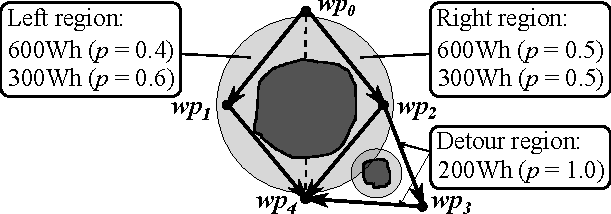
\includegraphics[width=0.82\columnwidth]{figures/phm_dm_example_v2.pdf}
	\caption{PHM vs. DM for a controlled system (Example \ref{ex:phm_dm})}
	\label{fig:phm_dm_example}
\end{figure}

\begin{figure}[h!]
	\centering
		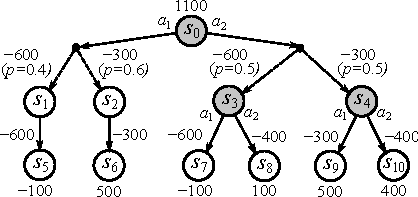
\includegraphics[width=0.9\columnwidth]{figures/phm_dm_tree_compact.pdf}
	\caption{Execution scenarios in Example \ref{ex:phm_dm}}
	\label{fig:phm_dm_tree}
\end{figure}

A decision support PHM algorithm, running a sufficiently large number of simulations, would consider two possible execution scenarios along the left route: (L1) $e_\text{total}=\unit[1200]{Wh}$, $p=0.4$ and (L2) $e_\text{total}=\unit[600]{Wh}$, $p=0.6$ ($e_\text{total}$ is the total energy consumed in a scenario). The expected energy consumption along the left route can then be computed as $E[e_\text{total, L}]=\unit[1200]{Wh} \cdot 0.4 + \unit[600]{Wh} \cdot 0.6 = \unit[840]{Wh}$.

The algorithm would then consider four possible execution scenarios along the right route (assuming uniform random choice of action at $wp_3$): (R1) $e_\text{total}=\unit[1200]{Wh}$, $p=0.25$; (R2) $e_\text{total}=\unit[600]{Wh}$, $p=0.25$; (R3) $e_\text{total}=\unit[1000]{Wh}$, $p=0.25$; and (R4) $e_\text{total}=\unit[700]{Wh}$, $p=0.25$. Then $E[e_\text{total, R}]=\unit[(1200+600+1000+700) \cdot 0.25]{Wh} = \unit[875]{Wh}$. With $E[e_\text{total, L}] < E[e_\text{total, R}]$, the PHM algorithm commits to the left path. Note that in many cases prognostics algorithms generate even less information to support action selection than what was done here (typically $p(\text{EOL})$ only).

A DM algorithm capable of sequential reasoning under uncertainty \cite{Kochenderfer2015} would compute $E[e_\text{total, L}] = \unit[840]{Wh}$ in the same manner as the PHM algorithm, as there are no actions needing to be selected along the left route after $wp_0$. On the right side, however, the DM algorithm can make an informed choice at $wp_2$, based on observations made along $wp_0 \rightarrow wp_2$. This implies having only two possible execution scenarios: (R1) if the terrain is observed as \textit{difficult}, the detour through $wp_3$ is taken, and (R2) if the terrain is observed as \textit{moderate}, the rover goes directly to $wp_4$. For R1, $e_\text{total}=\unit[1000]{Wh}$, $p=0.5$. For R2, $e_\text{total}=\unit[600]{Wh}$, $p=0.5$. The expected energy use is thus $E[e_\text{total, R}]=\unit[(1000+600) \cdot 0.5]{Wh} = \unit[800]{Wh}$. With $E[e_\text{total, L}] > E[e_\text{total, R}]$, the algorithm chooses the right path.

Now let us assume that the true terrain condition both on the left and the right sides of the crater is \textit{difficult}. The left path ($wp_0 \rightarrow wp_1 \rightarrow wp_4$) will require $\unit[1200]{Wh}$ to traverse, therefore a rover relying on the PHM algorithm will fall $\unit[100]{Wh}$ short and will not reach $wp_4$. A rover relying on the DM algorithm will expend only $\unit[1000]{Wh}$ (scenario R1), arriving at $wp_4$ with $\unit[100]{Wh}$ in reserve.

It may be suggested that the issues with the PHM approach could be eliminated if access to a precomputed operational policy $\pi_\text{DM}$ is provided. However, even if such a policy was available, that would still be insufficient. If, at time $t$, $p(\text{EOL})$ is computed using $\pi_\text{DM}$, then $a_{t+1,\text{SHM}}$ is taken on the basis of $p(\text{EOL})$, $p(\text{EOL})$ could immediately become invalid unless $T(s_t,a_{t+1,\text{SHM}}, s_{t+1}) = T(s_t,a_{t+1,\text{DM}}, s_{t+1})$.




